\documentclass{beamer}

% Tips:
% 1. create a Latex macro to make your job faster
\usepackage{subcaption}
\usepackage{hyperref}
\usepackage{tikz} % Include this in the preamble
\usetheme{Warsaw}
% \usetheme[progressbar = frametitle]{metropolis}
% \definecolor{UCcolor}{rgb}{0.82, 0.1, 0.26}
\definecolor{UCcolor}{rgb}{0.7, 0.0, 0.2}

\newcommand{\bluepause}{\addtocounter{beamerpauses}{-1}\color<+>{blue}}

\setbeamertemplate{frame numbering}[fraction]

\useoutertheme[subsection=false]{miniframes}
\usecolortheme[named=UCcolor]{structure}
% beamer themes: https://mpetroff.net/files/beamer-theme-matrix/

\logo{%
    \begin{tikzpicture}[remember picture, overlay]
        % Bottom left logo
        \node[anchor=south west, xshift=0.5cm, yshift=0.5cm] at (current page.south west) {
            
\includegraphics[width=2cm]{assets/imgs/uc_logo.png}
        };
        % Bottom right logo
        \node[anchor=south east, xshift=0.5cm, yshift=0.55cm] at (current page.south east) {
            
\includegraphics[width=2cm]{assets/imgs/download2.jpg}
        };
    \end{tikzpicture}
}

\title[Roads]{Effect of Road Maintenance on Housing Values, Employment and Wages}
% \subtitle{}
\author{David Brasington, Saani Rawat}
\institute{University of Cincinnati}
\date{8 Oct 2024}

\begin{document}

% Titlepage
\begin{frame}
\titlepage
\end{frame}

% Slide 1
% \begin{frame}[t]{Outline}\vspace{10pt}
% \begin{block}{Presentation preview}

% 1. Background

% 2. Motivation

% 3. Experiment Design

% 4. Results 

% 5. Assumption testing

% \end{block}
% \end{frame}

\section{Introduction}

\begin{frame}{Background}
% \frametitle{}
% % How are roads maintained in the US? 

Roads are important for economic well-being.

% % \begin{itemize}
% %     \item FEderLocal governments are responsible for maintaining roads 
% %     \item Local governments can levy taxes to fund road maintenance 
% %     \item Local governments can also issue bonds to fund road maintenance 
% %     \item Local governments can also receive federal and state grants to fund road maintenance 

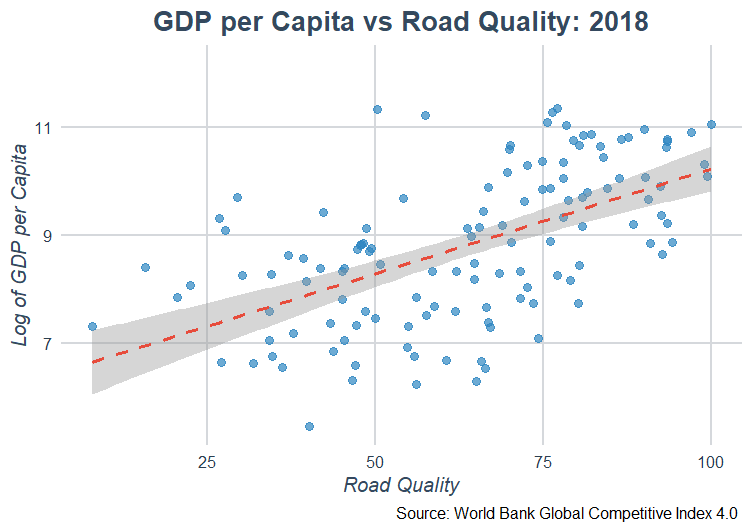
\includegraphics[width=9cm]{assets/imgs/road_quality_vs_gdp_per_cap.png}

\end{frame} 

\begin{frame}{Background}
    % \frametitle{}
    How are roads maintained in the US? 
        
    \begin{itemize}
        \item Gas taxes: Federal (\$0.18 per gallon) and State (\$0.38 per gallon for Ohio)
        \item Federal Grants and State funds for new projects and highways
        \item Vehicle registration fees, License plate fees, tolls and "user" taxes
        \item Local governments can use local tax revenue collected from property and income taxes to fund road maintenance
        \item 
    \end{itemize}
    % 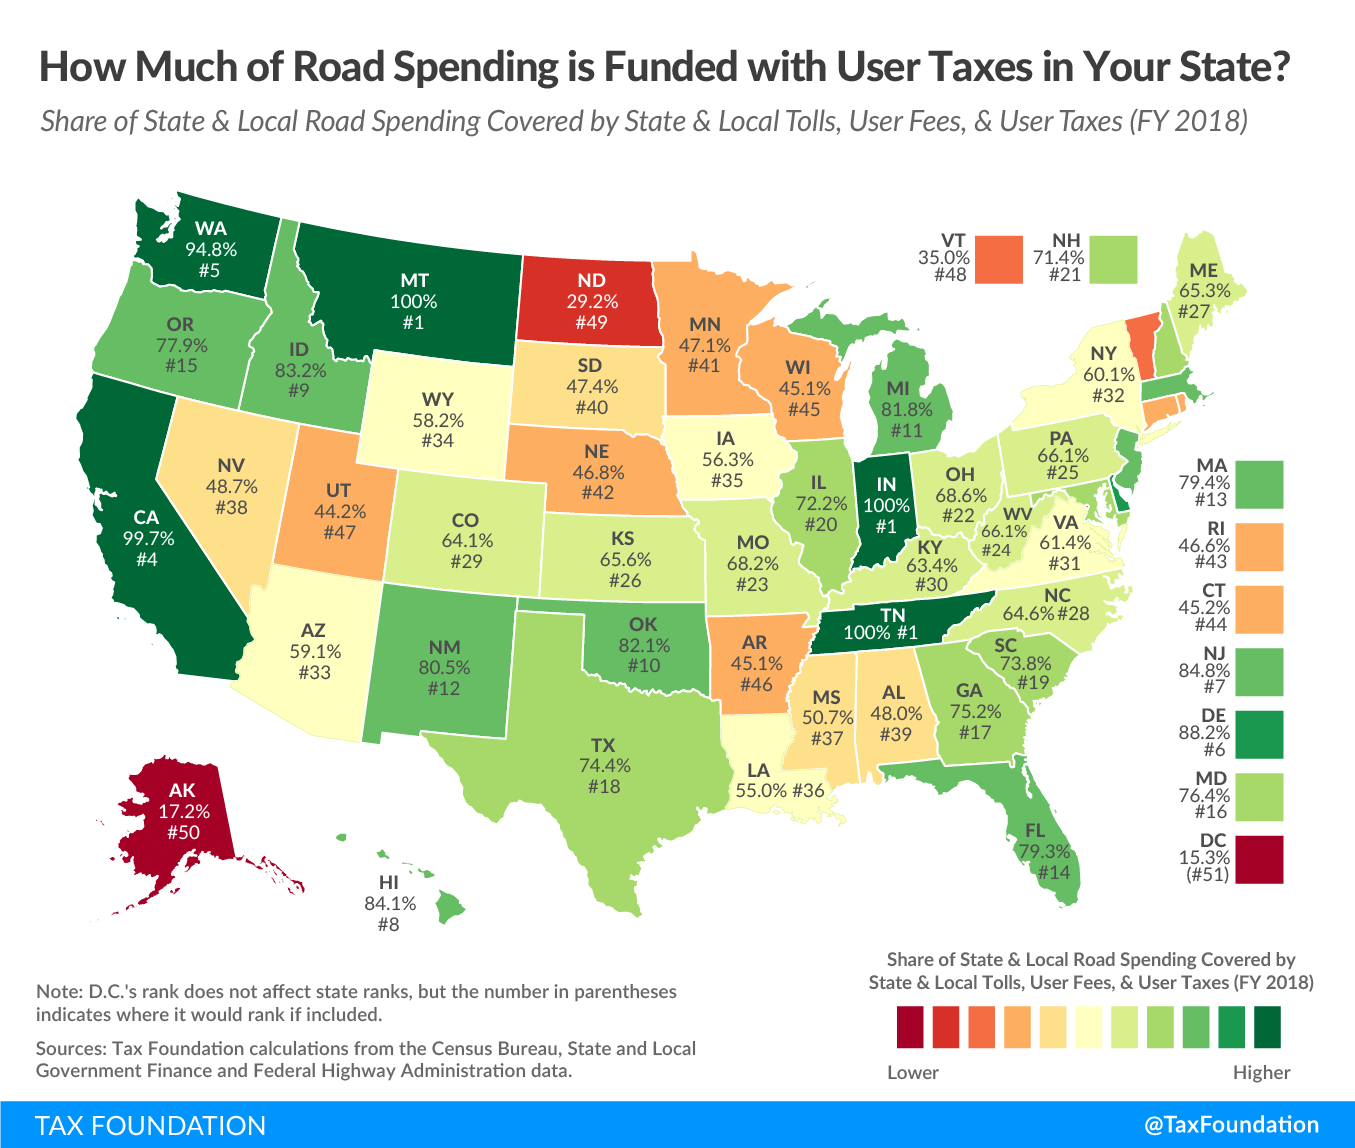
\includegraphics[width=9cm]{assets/imgs/road_spending_funding_us.png}
    
\end{frame} 

\begin{frame}{Background}
    % \frametitle{}
    How are roads maintained in Ohio? 
        
    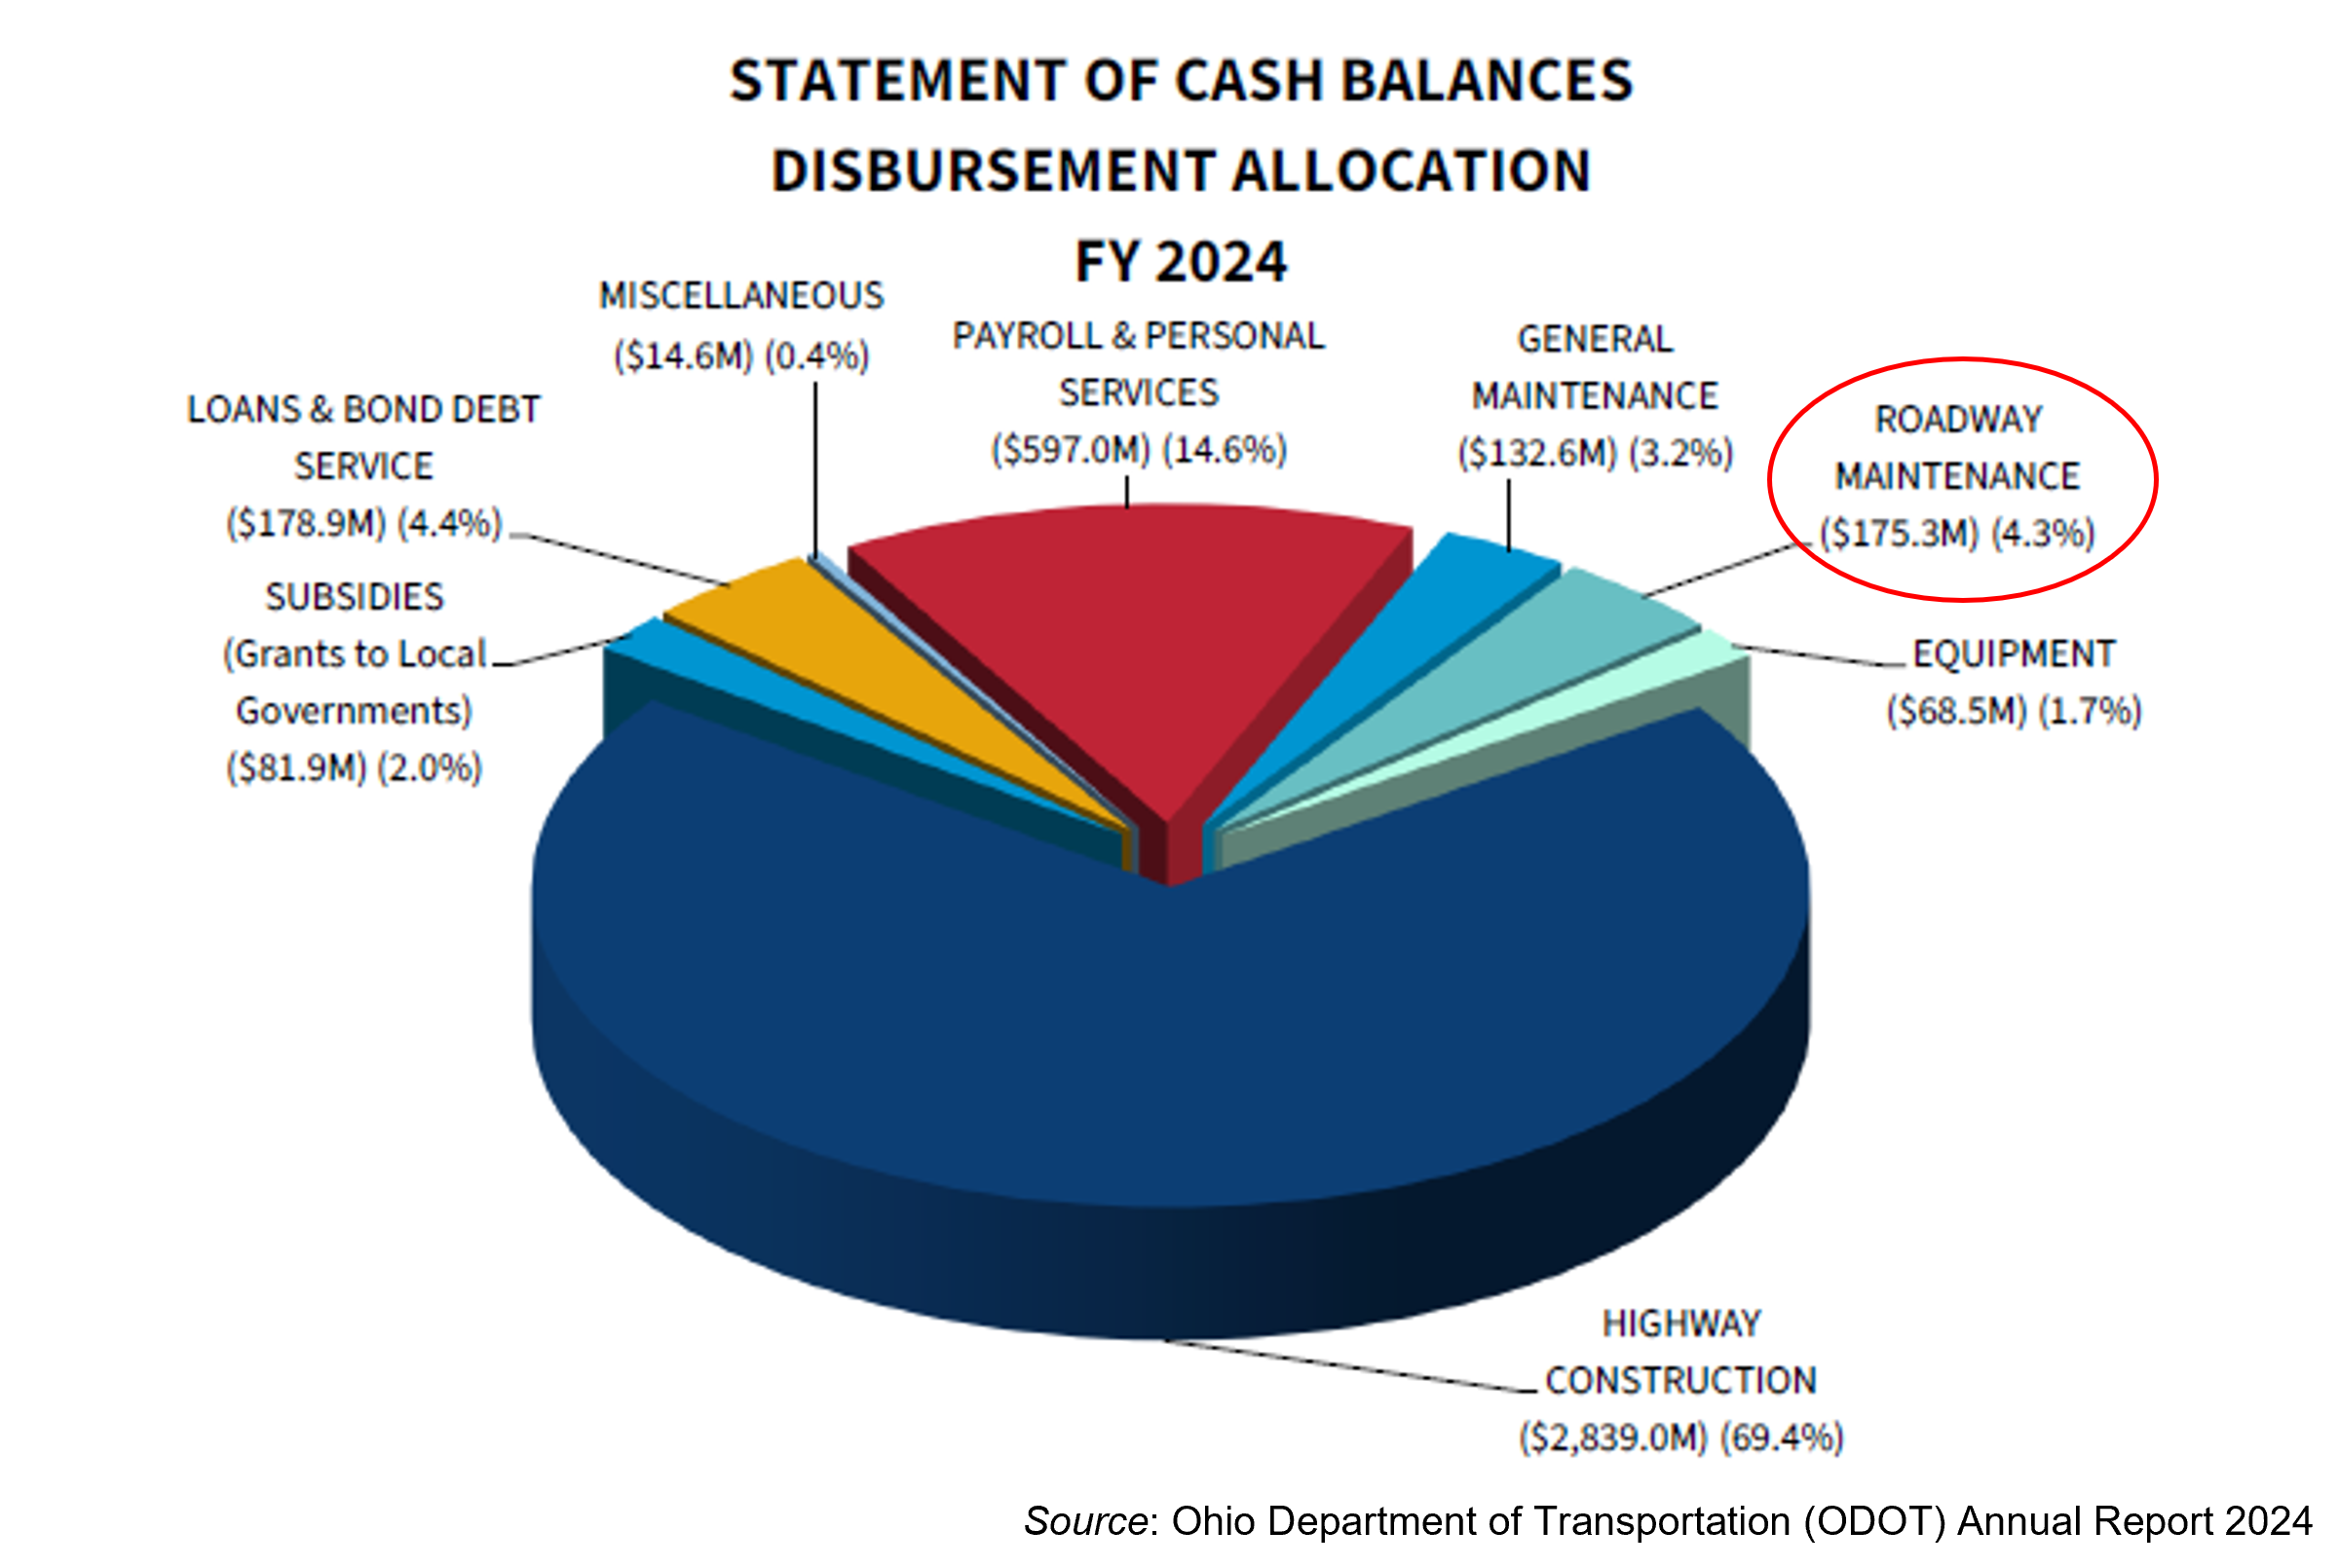
\includegraphics[width=9cm]{assets/imgs/odot_exp_2024.png}
    
\end{frame} 

\begin{frame}{Background}
    % \frametitle{}
    How are roads maintained in Ohio? 
        
    \begin{itemize}
        \item Only 4\% of ODOT budget is spent on road maintenance
        \item ODOT manages state highways and interstates
        \item Local roads maintained by townships and cities using local tax revenue (income and property taxes)
        \item \textcolor{red}{Townships and municipalities can propose local road levies, which are property tax assessments specifically earmarked for road maintenance and improvements. These levies must be approved by voters}
    \end{itemize}
    % 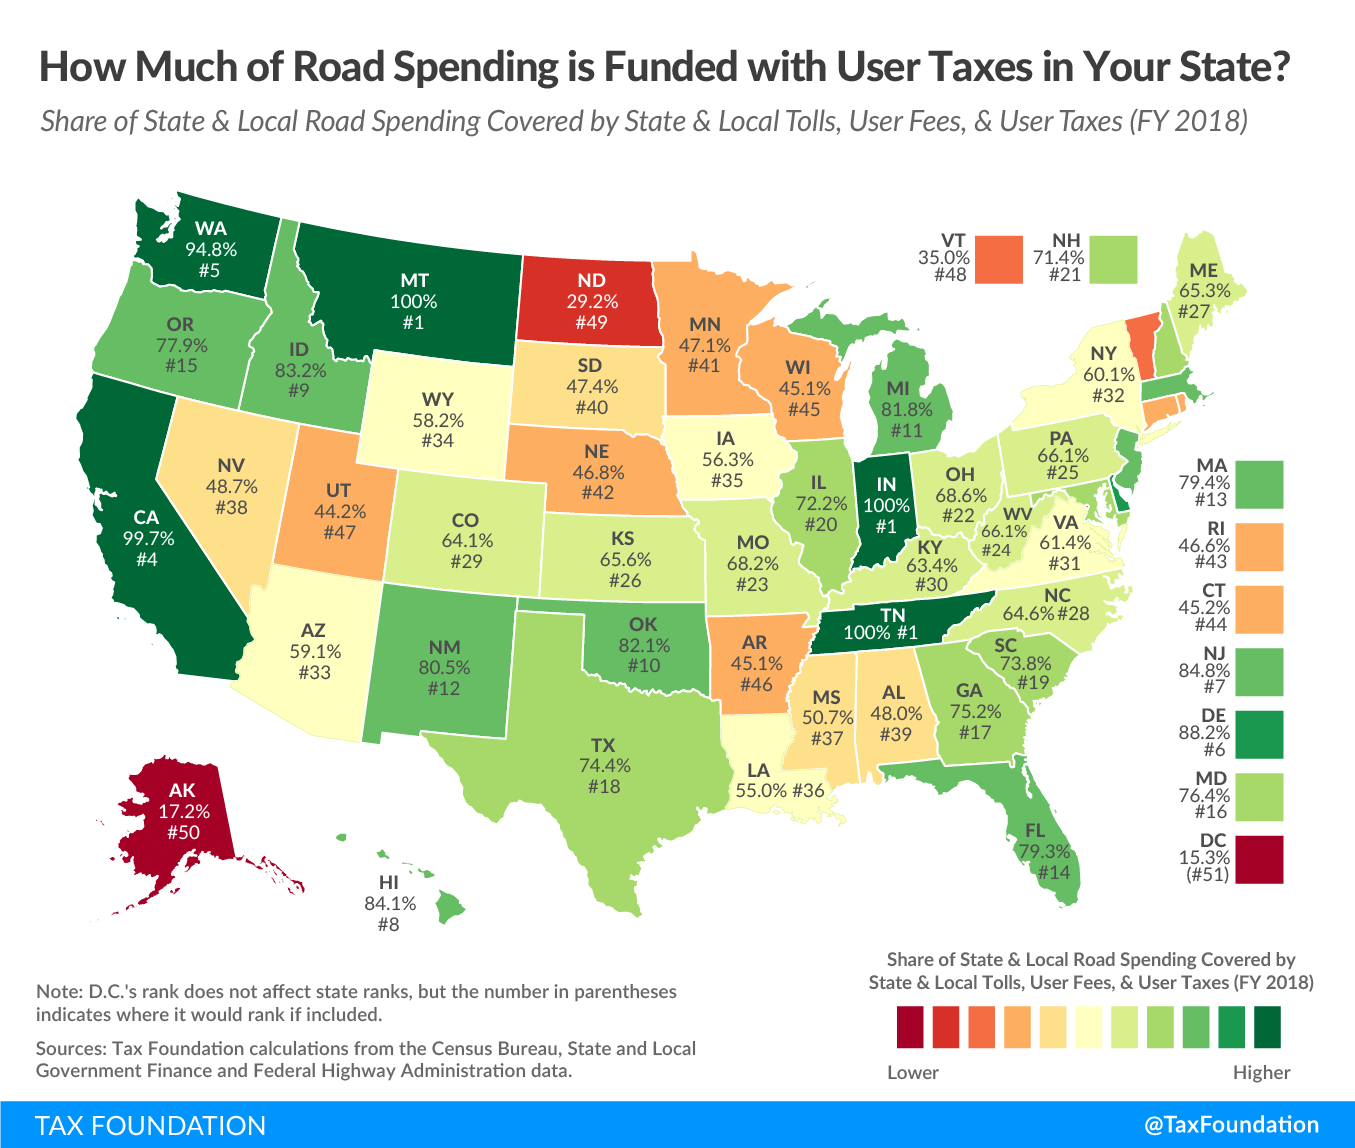
\includegraphics[width=9cm]{assets/imgs/road_spending_funding_us.png}
    
\end{frame} 

\begin{frame}{Motivation}
\frametitle{}

\underline{Natural experiment}: Local road maintenance tax levies that just pass or fail a road levy vote

\end{frame}

\begin{frame}{Research Question}
        \frametitle{}
        Do poorly maintained roads lead to a reduction in property values, employment and wages?
        
\end{frame}

\begin{frame}{Diagram of Thought Process} 
\frametitle{}
% \begin{minipage}{0.3\textwidth}
        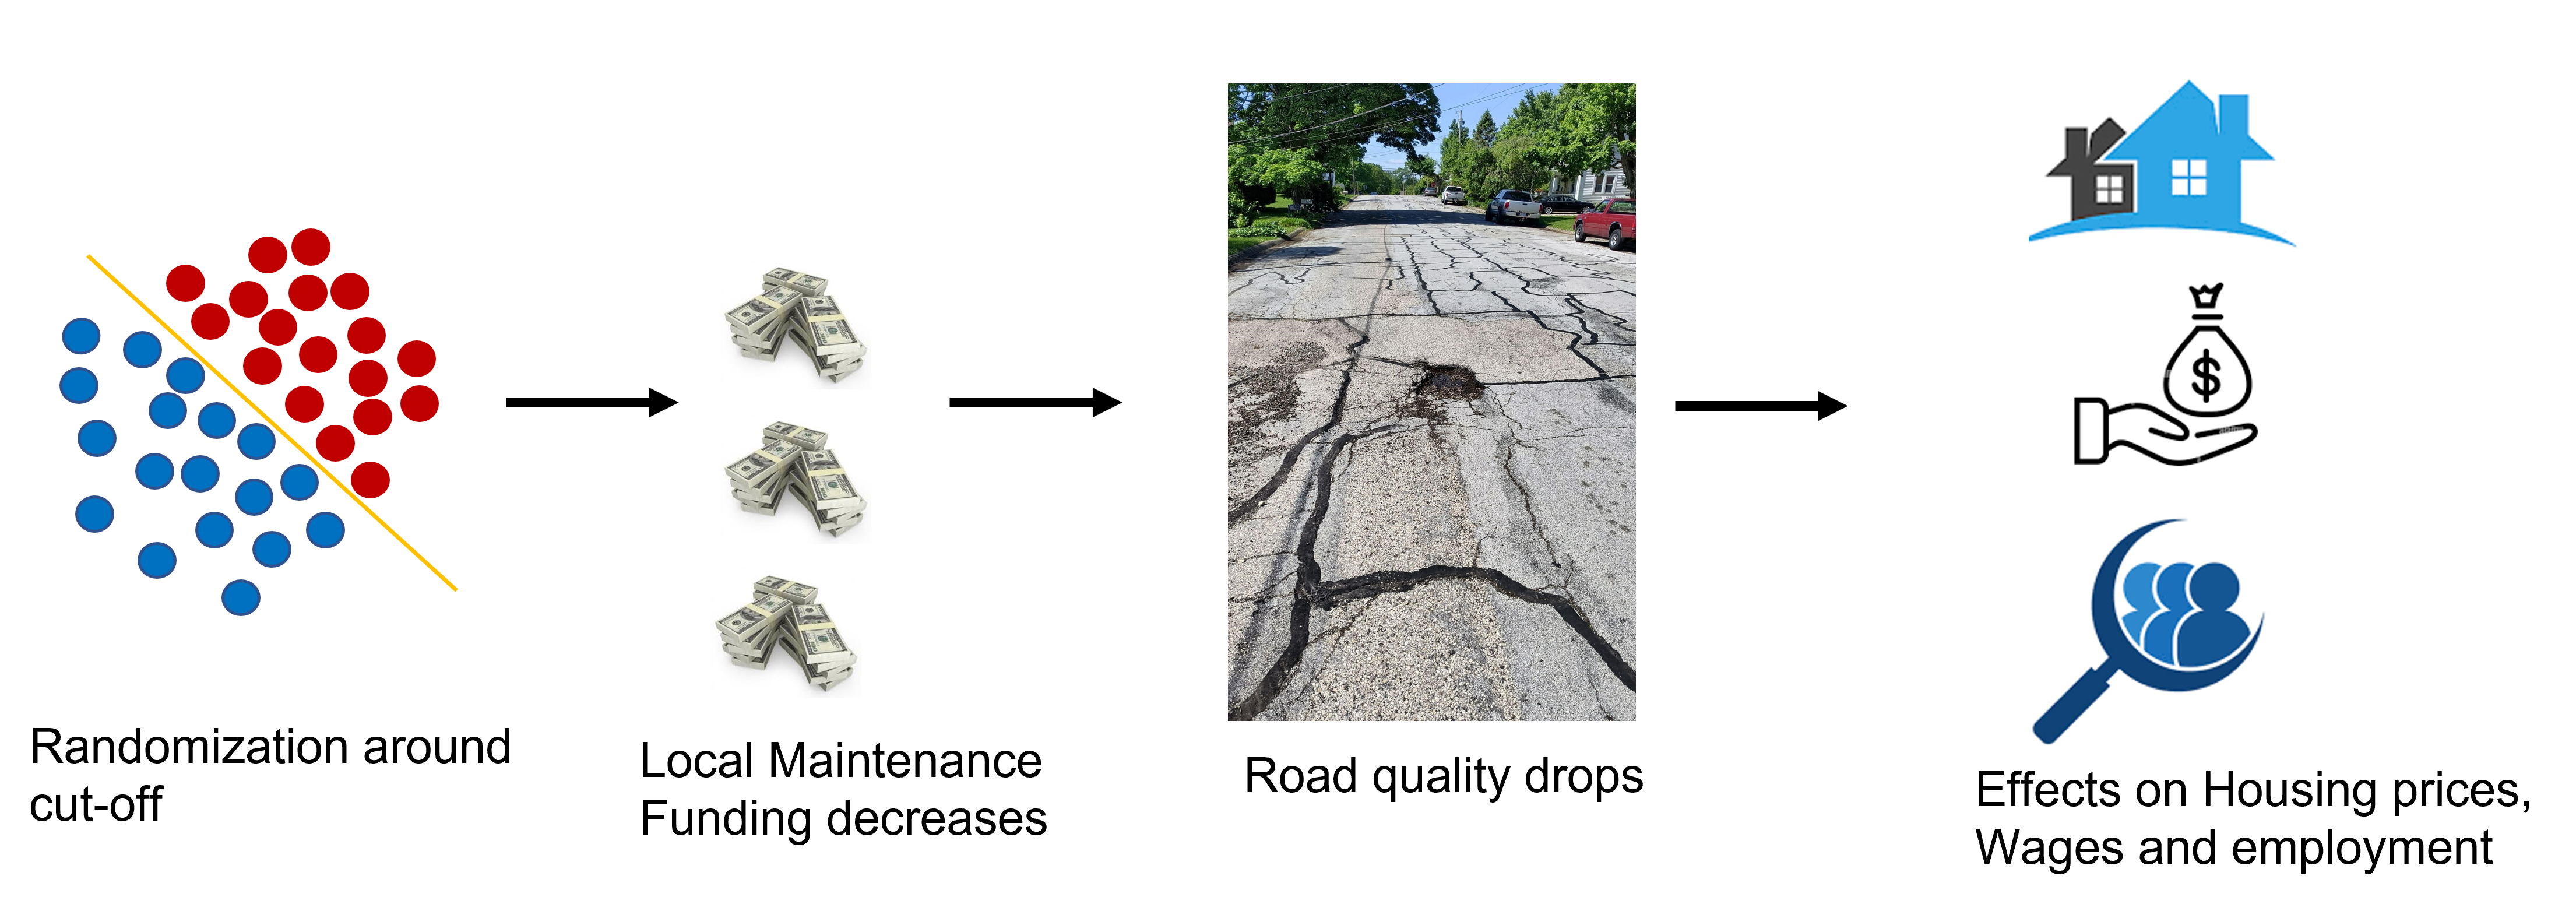
\includegraphics[width=11cm]{assets/imgs/thought_process.png}
% \end{minipage}%
% \begin{minipage}{0.5\textwidth}
%         % Your content here

% \end{minipage}
\end{frame}

\begin{frame}{Preview of Results}
\frametitle{}

\begin{itemize}
    \item Cities that cut road maintenance spending see a decline in property values of \$20,729 relative to similar cities that renewed funding, starting at four years after the vote.
    \item Houses in urban areas declined more than houses in rural areas.
    \item More expensive houses saw a larger decline in property values than cheaper houses.    
    \item High-poverty cities that cut road spending have 11\% lower employment compared to similar cities that renewed funding and \%17.8 lower wages.    
\end{itemize}
        
\end{frame}

\begin{frame}{Contribution}
\frametitle{}

\begin{itemize}
    \item While most of the research has focused on effects of new infrastructure (new highways, trains etc.), we show long-term effects of road maintenance on different economic outcomes in a developed economy.
    \item We aim to develop a novel road quality index using  a Machine Learning model - Convolutional Neural Networks (CNN) to measure road quality.
    % \item 
\end{itemize}

\end{frame}
        

\section{Literature Review}

\begin{frame}{Literature Review: Roads and Economic Outcomes}
\frametitle{}

\begin{itemize}
\label{main_lit}    
    \item New road projects - 

    {\small
    {\bf Asher and Novosad (2020)}: India
    
    {\bf Shamdasani (2021)}: India
    
    {\bf Mu and Van De Walle (2010)}: Vietnam    
    }
    
    \item Road quality measurement -

    {\small
    {\bf Currier, Glaeser \& Kreindler (2023)}: using vertical acceleration data from smartphones

    {\bf Brewer et al (2021)}: use satellite images to measure road quality

    }    
    
\end{itemize}

For more details, see the slides on \hyperlink{lit_background}{\beamerbutton{more literature}}.
\end{frame}

\section{Data}

\begin{frame}{Taxation and Housing Data}
\frametitle{}
    \label{data}
    \begin{block}{Sources:}
    1. Ohio Secretary of State's Office
    
    2. CoreLogic
    
    3. U.S. Census Bureau
    \end{block}
    % \pause
    
    \begin{block}{Period:}
    1991-2021
    \end{block}
    % \pause
    
    \begin{block}{Variables:}
    Dependent variable: Sale amount of a property in county subdivision (or village) i and period t
    
    Running variable: \% Votes in favor for renewal of a road tax levy. Cutoff = 50\%
    
    Covariates: Village-specific characteristics \hyperlink{variables}{\beamerbutton{Specific Variables}}
    \end{block}
    
\end{frame}

% \begin{frame}{Spending Data}
% \frametitle{}
% \end{frame}

\begin{frame}{Spending \& Road quality Data}
    \frametitle{}
    
    \begin{block}{Spending:}
        % Add content related to spending here
        Sunshine Law, OH: Ohio Auditor's report by Ohio Auditor of State
        \begin{itemize}
            \item After a tax cut, average drop in cash disbursements for road maintenance is 34\%
            \item We are working on other measures of road maintenance spending deduction
            % \item 
        \end{itemize}        
    \end{block}

    \begin{block}{Road Quality:}
        % Add content related to road quality here
        \begin{itemize}
            \item Google Earth and Google Street Maps
            \item Ethan Brewer's road quality data buffet
            % \item 
        \end{itemize}        
    \end{block}


\end{frame}

\begin{frame}{Andover vs Morgan: A Tale of Two Townships in Ashtabula County, OH}
    \frametitle{}
    \begin{table}[ht]
        \centering
        % \caption{County Subdivisions with Most Successful and Failed Renewals}
        \label{tab:ash_tale}
        \begin{tabular}{p{1cm}p{1.5cm}p{1cm}ccp{1.5cm}}
            \hline
            \scriptsize County Subdivision & \scriptsize Subdivision Type & \scriptsize County & \scriptsize Renewals & \scriptsize Cuts & \scriptsize Percent Cut \\      \hline
            % \multicolumn{6}{l}{\scriptsize \textbf{Panel A. Maximum number of successful renewals}} \\
            \scriptsize Andover & \scriptsize Township & \scriptsize Ashtabula & \scriptsize 16 & \scriptsize 0 & \scriptsize 0\% \\
            \\
            % \multicolumn{6}{l}{\scriptsize \textbf{Panel B. Maximum number of failed renewals}} \\
            \scriptsize Morgan & \scriptsize Township & \scriptsize Ashtabula & \scriptsize 7 & \scriptsize 9 & \scriptsize 56\% \\
            \hline       \end{tabular}
    \end{table}
\end{frame}

\begin{frame}{Andover vs Morgan: A Tale of Two Townships in Ashtabula County, OH}
    \frametitle{}

\begin{figure}[htbp]
    \centering
    \begin{minipage}[b]{0.49\textwidth}
        \centering
        \begin{subfigure}[b]{\textwidth}
            \centering
            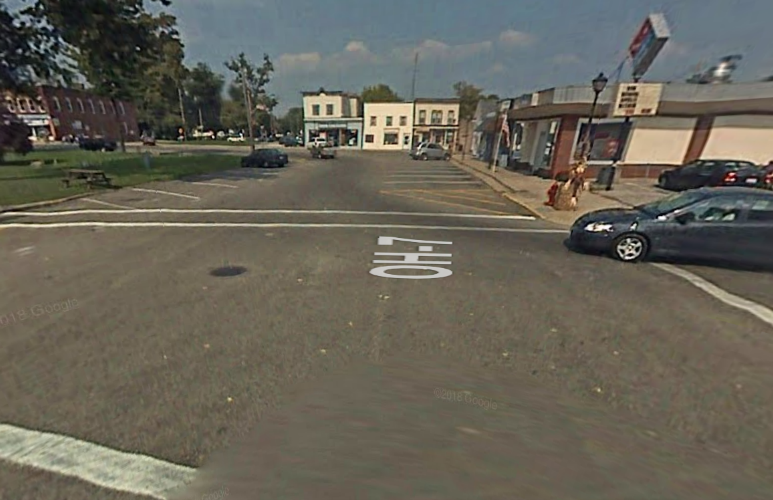
\includegraphics[width=\textwidth,keepaspectratio]{assets/imgs/andover_township_14grandarmy_2007.png}
            \caption{Grand Army of the Republic Hwy: 2007
            \label{fig:andover_2007}}
        \end{subfigure}
    \end{minipage}
    \hfill
    \begin{minipage}[b]{0.49\textwidth}
        \centering
        \begin{subfigure}[b]{\textwidth}
            \centering
            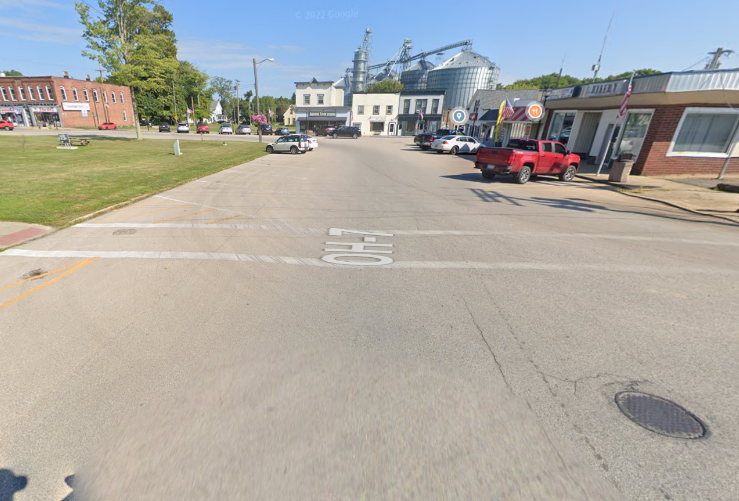
\includegraphics[width=\textwidth,keepaspectratio]{assets/imgs/andover_township_14grandarmy_2022.png}
            \caption{Grand Army of the Republic Hwy: 2022}
            \label{fig:andover_2022}
        \end{subfigure}
    \end{minipage}

    % \vspace{1em}

    % \caption{Andover township - Road quality}
    % \label{fig:rd_andover}
\end{figure}

% \begin{figure}[htbp]
%     \centering
%     \begin{minipage}[b]{0.49\textwidth}
%         \centering
%         \begin{subfigure}[b]{\textwidth}
%             \centering
%             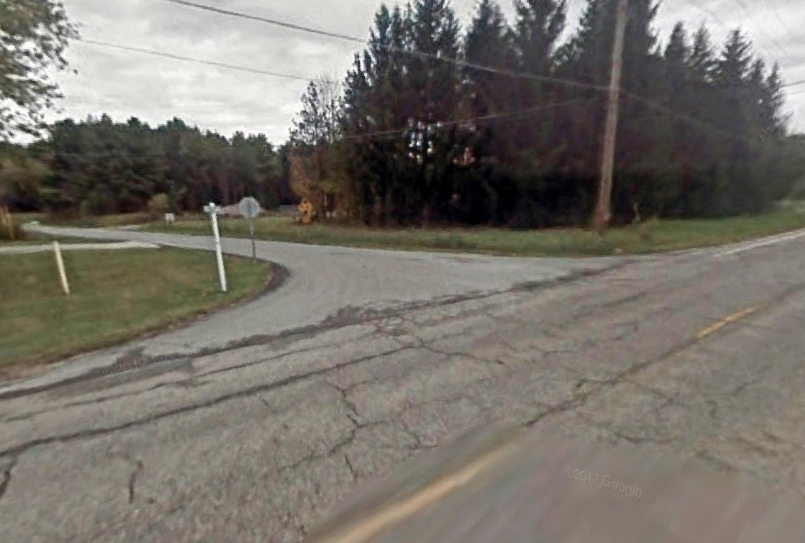
\includegraphics[width=\textwidth,keepaspectratio]{assets/imgs/morgan_township_2801OH-45_2009.png}
%             \caption{OH-45: 2009}
%             \label{fig:morgan_oh_2009}
%         \end{subfigure}
%     \end{minipage}
%     \hfill
%     \begin{minipage}[b]{0.49\textwidth}
%         \centering
%         \begin{subfigure}[b]{\textwidth}
%             \centering
%             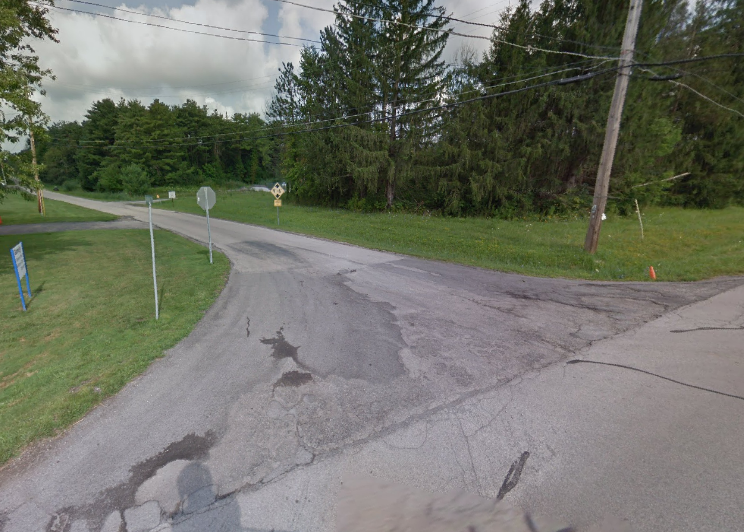
\includegraphics[width=\textwidth,keepaspectratio]{assets/imgs/morgan_township_2801OH-45_2018.png}
%             \caption{OH-25: 2018}
%             \label{fig:morgan_oh_2018}
%         \end{subfigure}
%     \end{minipage}        
    % \caption{Morgan township - Road quality}
    % \label{fig:rd_morgan}
% \end{figure}

\end{frame}

\begin{frame}{Andover vs Morgan: A Tale of Two Townships in Ashtabula County, OH}
    \frametitle{}

\begin{figure}[htbp]
    \centering
    \begin{minipage}[b]{0.49\textwidth}
        \centering
        \begin{subfigure}[b]{\textwidth}
            \centering
            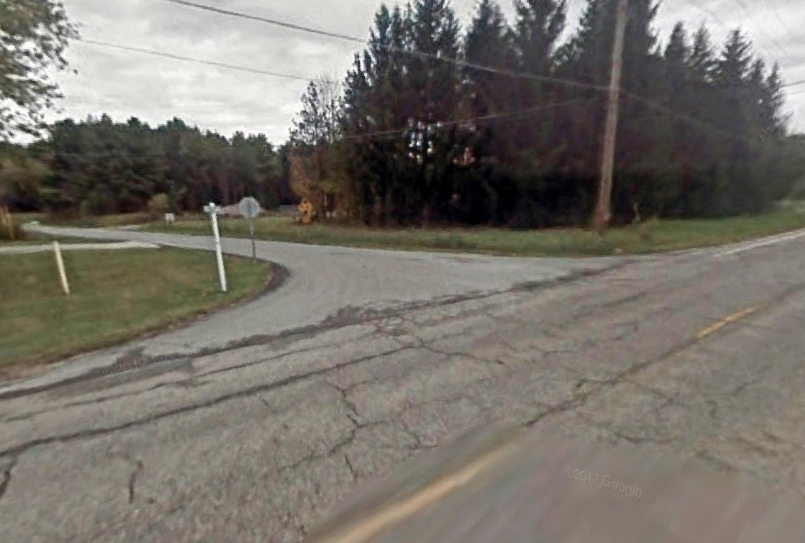
\includegraphics[width=\textwidth,keepaspectratio]{assets/imgs/morgan_township_2801OH-45_2009.png}
            \caption{OH-45: 2009}
            \label{fig:morgan_oh_2009}
        \end{subfigure}
    \end{minipage}
    \hfill
    \begin{minipage}[b]{0.49\textwidth}
        \centering
        \begin{subfigure}[b]{\textwidth}
            \centering
            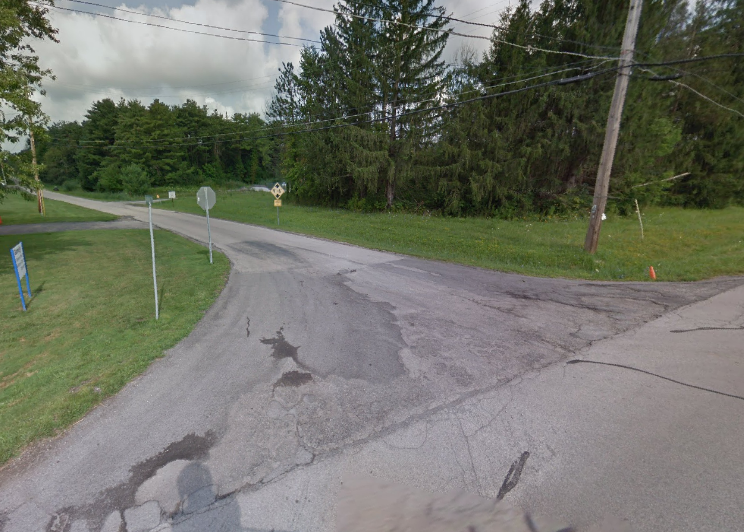
\includegraphics[width=\textwidth,keepaspectratio]{assets/imgs/morgan_township_2801OH-45_2018.png}
            \caption{OH-45: 2018}
            \label{fig:morgan_oh_2018}
        \end{subfigure}
    \end{minipage}        
    % \caption{Morgan township - Road quality}
    % \label{fig:rd_morgan}
\end{figure}

\end{frame}
        
\begin{frame}{Road Quality Index using CNN}
\frametitle{}
Currently, we are pursuing development of a measure for road quality using images from Google Earth and Google Street Maps.

\begin{itemize}
    \item Using 53,000 satellite images from roads in U.S, we leverage work from Ethan Brewer et al (2021) and use Google's InceptionV3 ML model. This model has been shown to have an out-of-sample prediction accuracy of 94\%.
    \item We plan to fine tune the model on Ohio specific images, and then use it to predict road quality in Ohio. 
\end{itemize}

\end{frame}

\begin{frame}{Road Quality Index using CNN}
    \frametitle{}
    Sample images from Google Earth, with poor (0), decent (1) and high (2) quality.

    \begin{figure}[htbp]
        \centering
        \begin{minipage}[b]{0.49\textwidth}
            \centering
            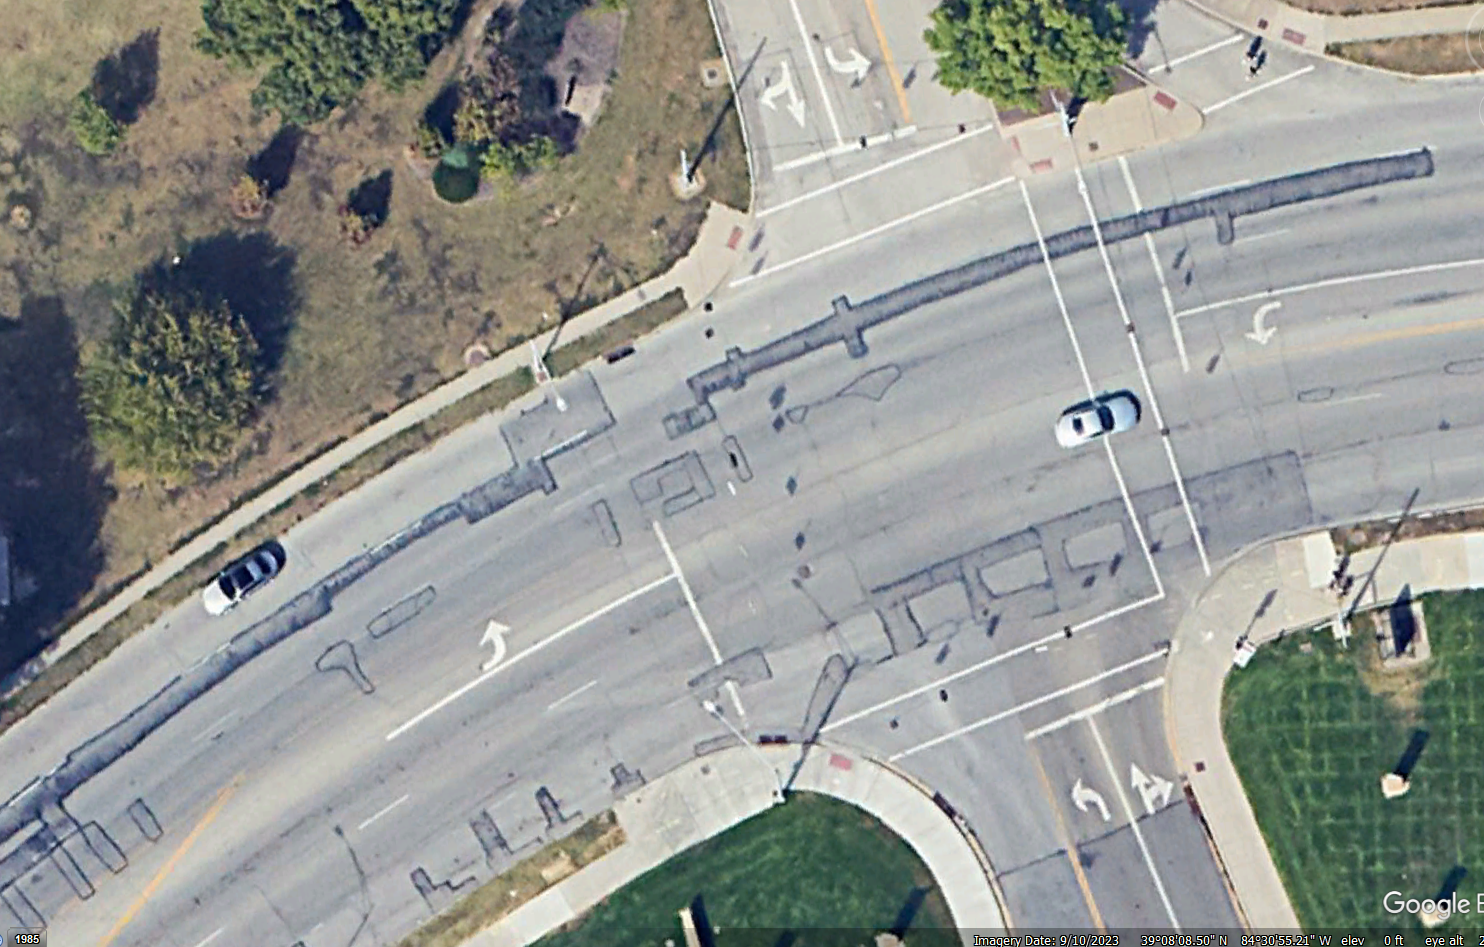
\includegraphics[width=\textwidth]{assets/imgs/mlk_bad.png}
            \caption{a "poor quality" road}
            \label{fig:image1}
        \end{minipage}
        \hfill
        \begin{minipage}[b]{0.49\textwidth}
            \centering
            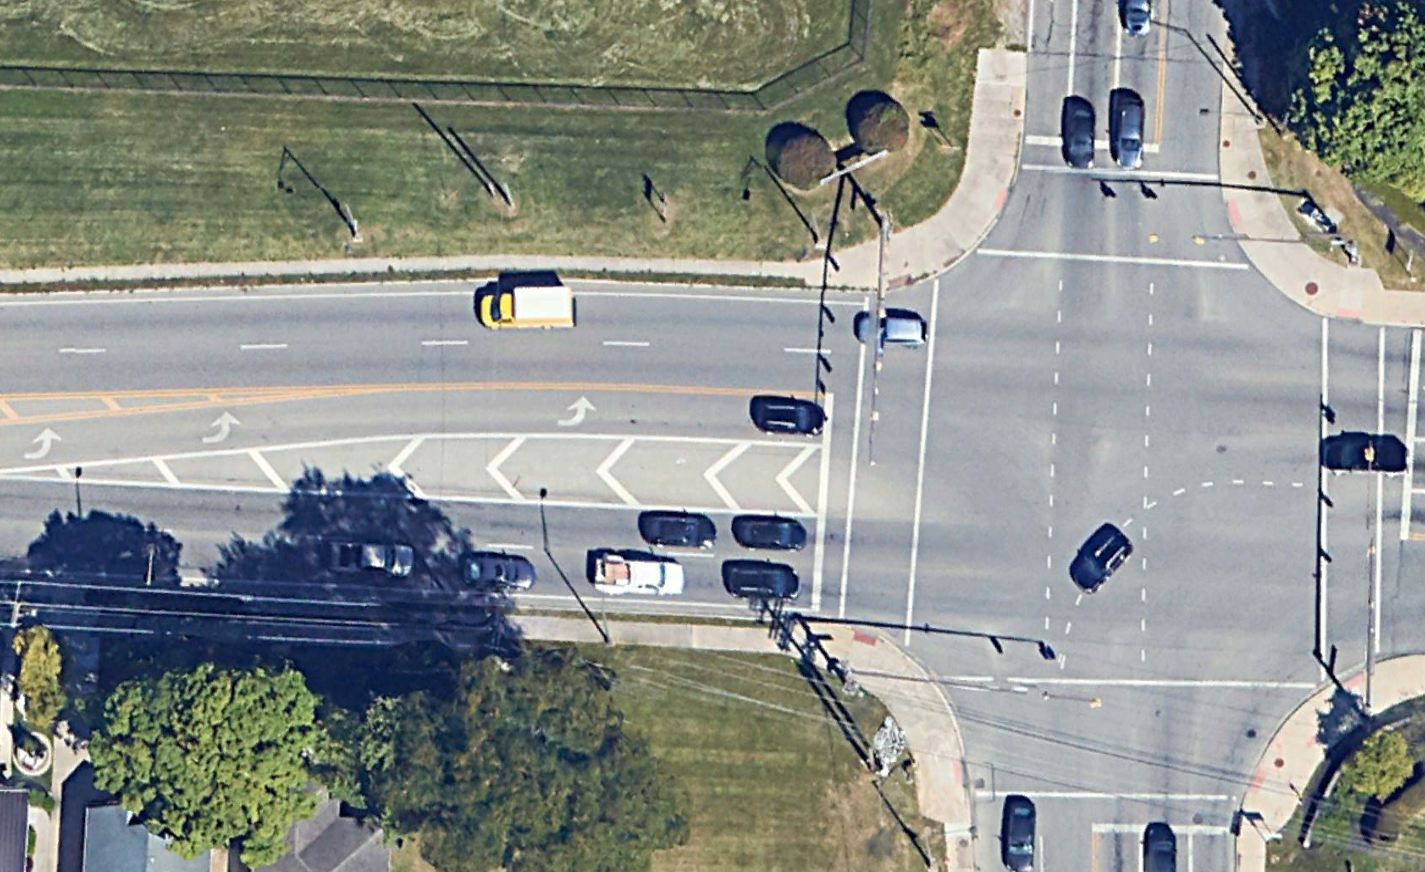
\includegraphics[width=\textwidth]{assets/imgs/road_good.png}
            \caption{a "high quality" road}
            \label{fig:image2}
        \end{minipage}
    \end{figure}
    

\end{frame}
     


\begin{frame}{RD plots}
    \frametitle{}
    \label{main_rd}

    \begin{figure}[htbp]
        \centering
        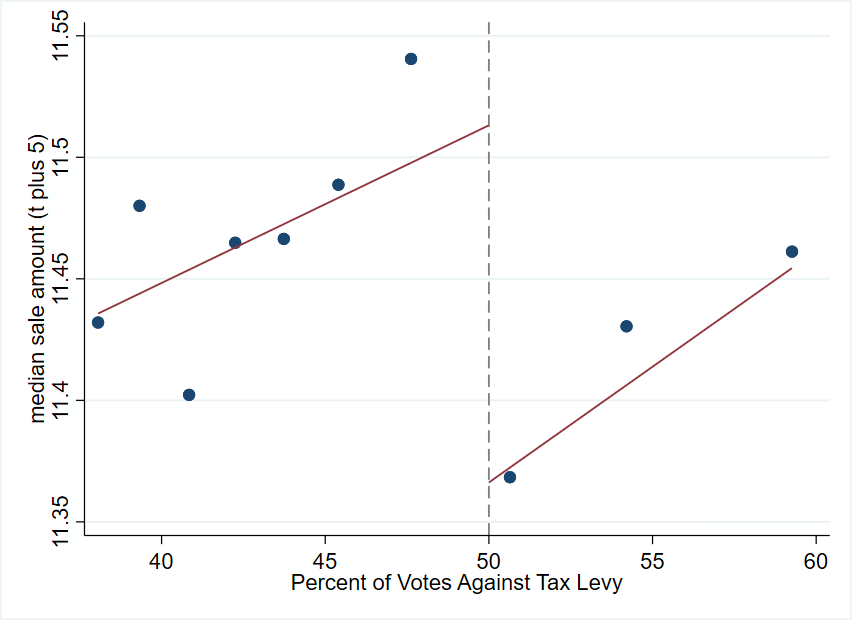
\includegraphics[width=0.8\textwidth]{assets/imgs/rd_plot_median_sale_amount_t_plus_5_tri_mserd_1_2_within.png}
        \caption{Log of Median Sale Amount: 5 years after the vote}
        \label{fig:rd_plot}
    \end{figure}

    \begin{center}
        \hyperlink{all_rd}{\beamerbutton{Housing Price: All RD plots}}
    \end{center}

\end{frame}

\section{Empirical Strategy}

% \begin{frame}[t]{Quasi-Experiment Design: getting a little "jumpy"}\vspace{3pt}
\begin{frame}{Quasi-Experiment Design: Regression Discontinuity}\vspace{3pt}
\begin{block}{Model equation}

{\normalsize $Y_{it} = \alpha + \textcolor{blue}{\tau} D_{it} + \beta_1 X_{it} + \beta_2 D_{it} X_{it} + \delta_1 W_{1it} + ... + \delta_k W_{kit} + \epsilon_{it}$}  , where

$i \in \{1 , ...., N \}, T \in \{1, ... , T \}$, for $N, T \in \mathbb{Z}_+$ 

$Y_{it} :$ economic outcome such as median sale amount of property, wages per worker, employment, for village i at time t 

$X_{it} :$ \% votes against for renewing a road tax levy for village i at time t  

$
D_{it}=\begin{cases} 1  &\text{, if \% votes against }  > 50 ,\\ 0 &\text{, if \% vote against }  \le 50 \end{cases}
$  

% $W_{kit}$: $k^{th}$ covariate for village i at time t 

% $\textcolor{blue}{\tau}:$ parameter of interest i.e. effect of passing a road tax levy on property sale amount

% $\epsilon_{it}$ is the purely random error
\end{block}
\end{frame}

\begin{frame}[t]{Quasi-Experiment Design: Regression Discontinuity}\vspace{10pt}
Specifications: 

\begin{itemize}
    \item bandwidth selection: mserd 
    \item kernel: triangular
    \item p: order of local polynomial for point estimator
    \item q: order of local polynomial for bias correction
\end{itemize}

\end{frame}

\section{Results}


\begin{frame}{Results: Median Housing Prices}
    \frametitle{}
    \begin{figure}[htbp]
        \centering
        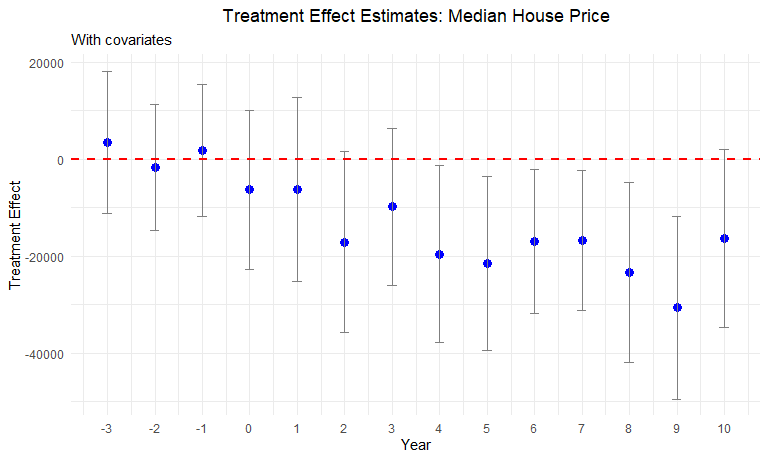
\includegraphics[width=0.8\textwidth]{assets/imgs/tes_gs.png}
        \label{fig:tes_gs}
    \end{figure}
\end{frame}

\begin{frame}{Results: Urban vs Rural}
    \frametitle{}
    \begin{figure}[htbp]
        \centering
        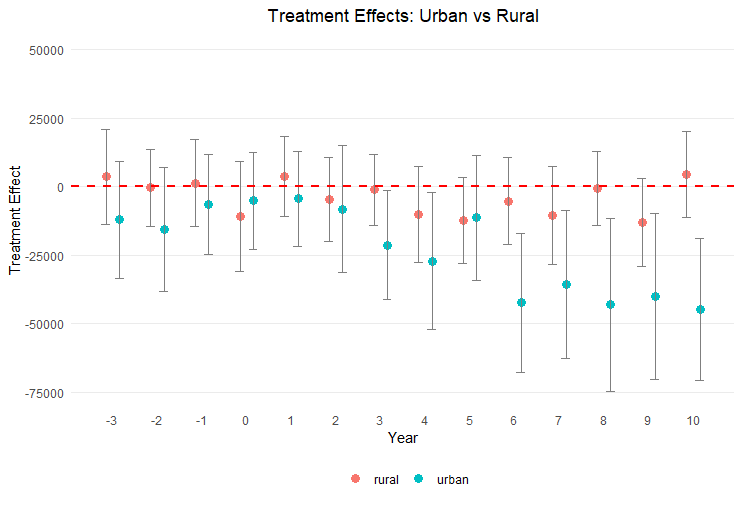
\includegraphics[width=0.8\textwidth]{assets/imgs/tes_covs_ua_new.png}
        % \caption{Event study: Urban vs Rural}
        \label{fig:tes_covs_ua}
    \end{figure}
\end{frame}

\begin{frame}{Results: Quantile Effect}
    \frametitle{}
    \begin{figure}[htbp]
        \centering
        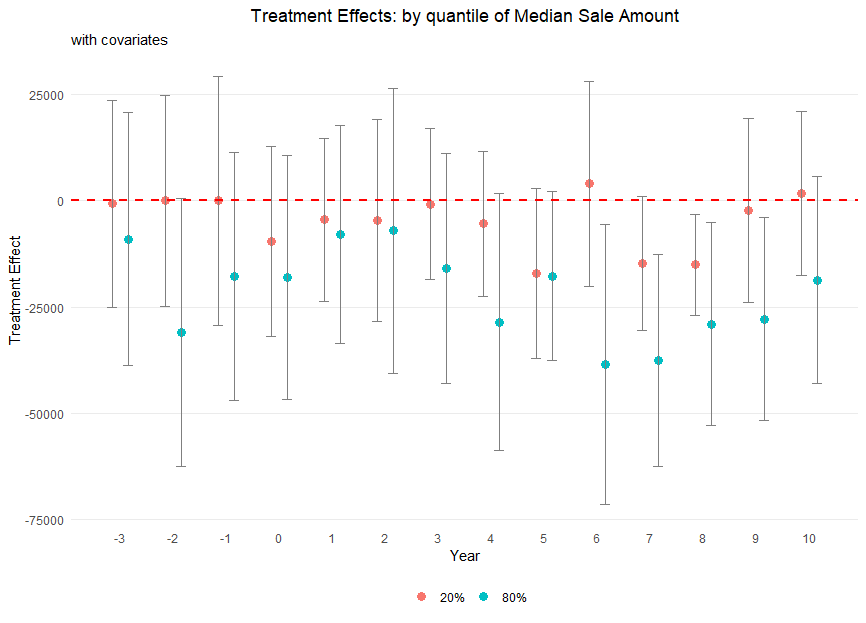
\includegraphics[width=0.8\textwidth]{assets/imgs/tes_qte_covs.png}
        % \caption{Event study: Urban vs Rural}
        \label{fig:tes_qte}
    \end{figure}
\end{frame}

\begin{frame}{Results: Wages per worker}
    \frametitle{}
    \begin{figure}[htbp]
        \centering
        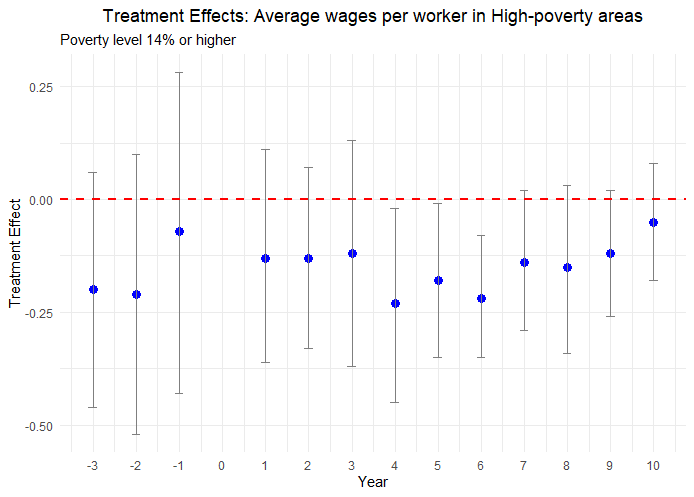
\includegraphics[width=0.8\textwidth]{assets/imgs/tes_wages_per_emp_hp.png}
        % \caption{Event study: Urban vs Rural}
        \label{fig:tes_wages}
    \end{figure}
\end{frame}

% \begin{frame}{Results}
%     \frametitle{}
% \end{frame}

\section{Appendix}

\begin{frame}
    \centering
    \Huge Appendix
\end{frame}

\begin{frame}{Housing: RD plots}
\frametitle{}
\label{all_rd}

\begin{figure}[htbp]
    \centering
    \begin{minipage}[b]{0.35\textwidth}
        \centering
        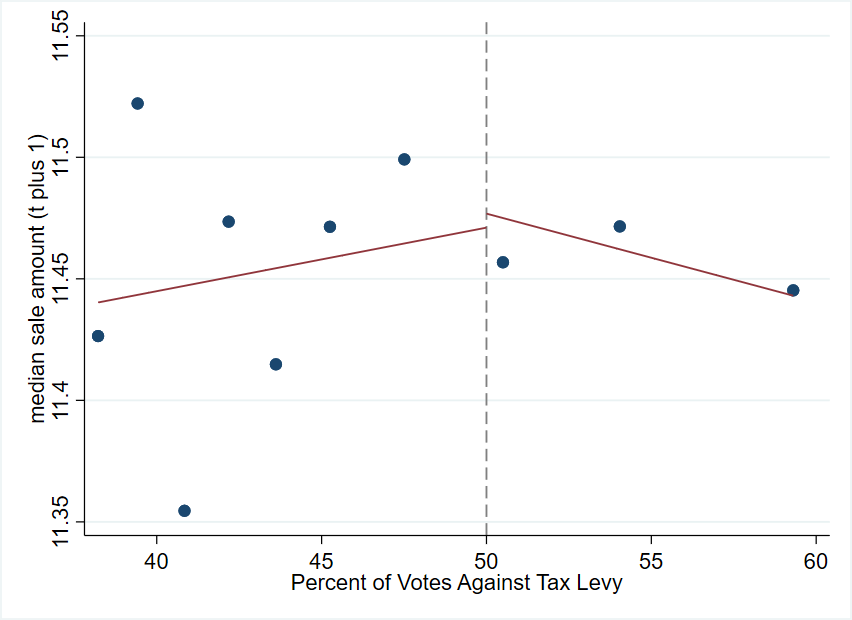
\includegraphics[width=\textwidth]{assets/imgs/rd_plot_median_sale_amount_t_plus_1_tri_mserd_1_2_within.png}
        \caption{Year 1 after vote}
        \label{fig:image1}
    \end{minipage}
    \hfill
    \begin{minipage}[b]{0.35\textwidth}
        \centering
        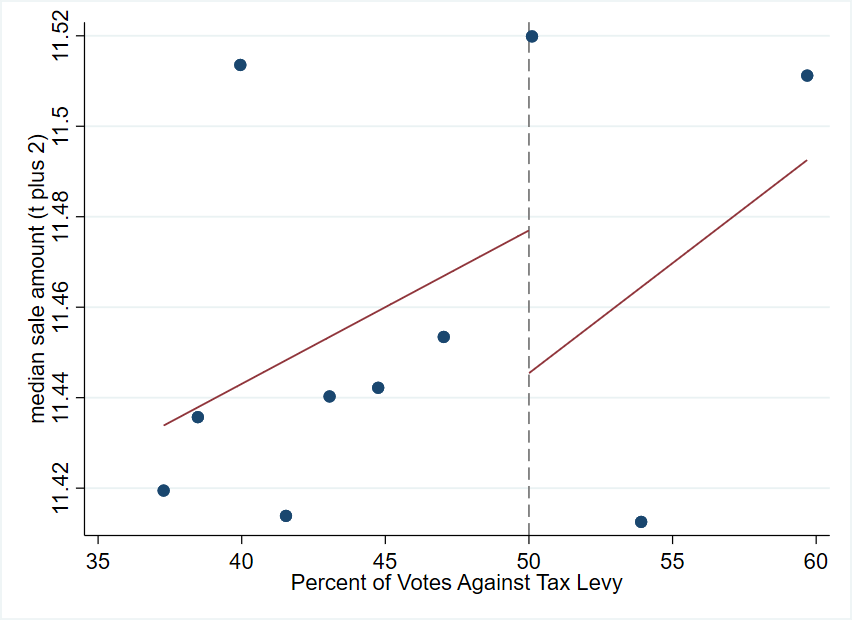
\includegraphics[width=\textwidth]{assets/imgs/rd_plot_median_sale_amount_t_plus_2_tri_mserd_1_2_within.png}
        \caption{Year 2 after vote}
        \label{fig:image2}
    \end{minipage}
    \vspace{1em}
    \begin{minipage}[b]{0.35\textwidth}
        \centering
        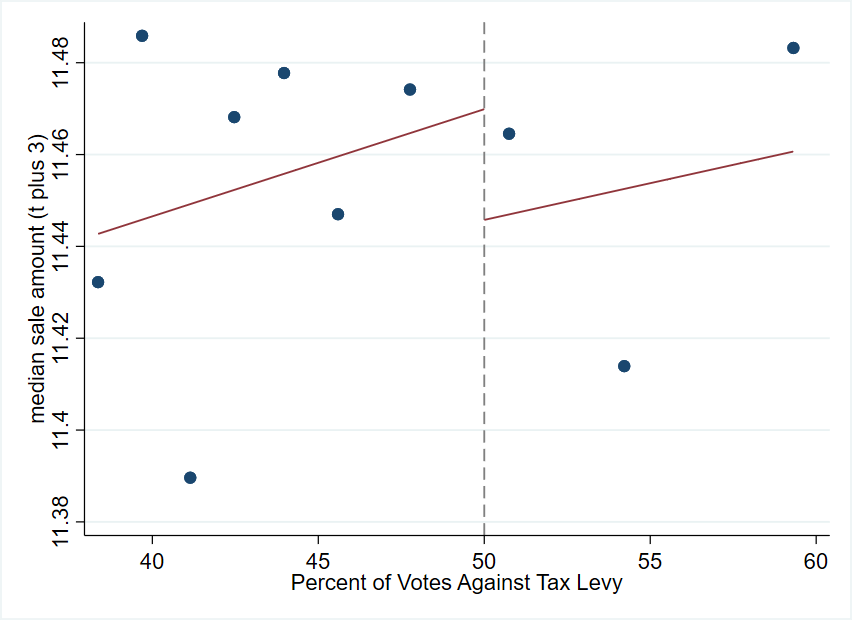
\includegraphics[width=\textwidth]{assets/imgs/rd_plot_median_sale_amount_t_plus_3_tri_mserd_1_2_within.png}
        \caption{Year 3 after vote}
        \label{fig:image3}
    \end{minipage}
    \hfill
    \begin{minipage}[b]{0.35\textwidth}
        \centering
        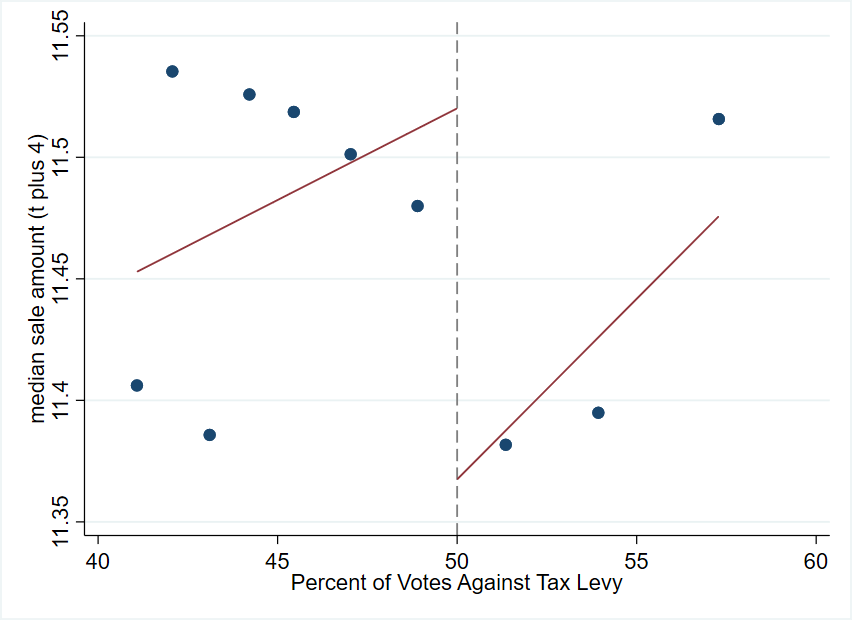
\includegraphics[width=\textwidth]{assets/imgs/rd_plot_median_sale_amount_t_plus_4_tri_mserd_1_2_within.png}
        \caption{Year 4 after vote}
        \label{fig:image4}
    \end{minipage}
\end{figure}

\end{frame}

\begin{frame}{Housing: RD plots}
    \frametitle{}
    
    \begin{figure}[htbp]
        \centering
        \begin{minipage}[b]{0.35\textwidth}
            \centering
            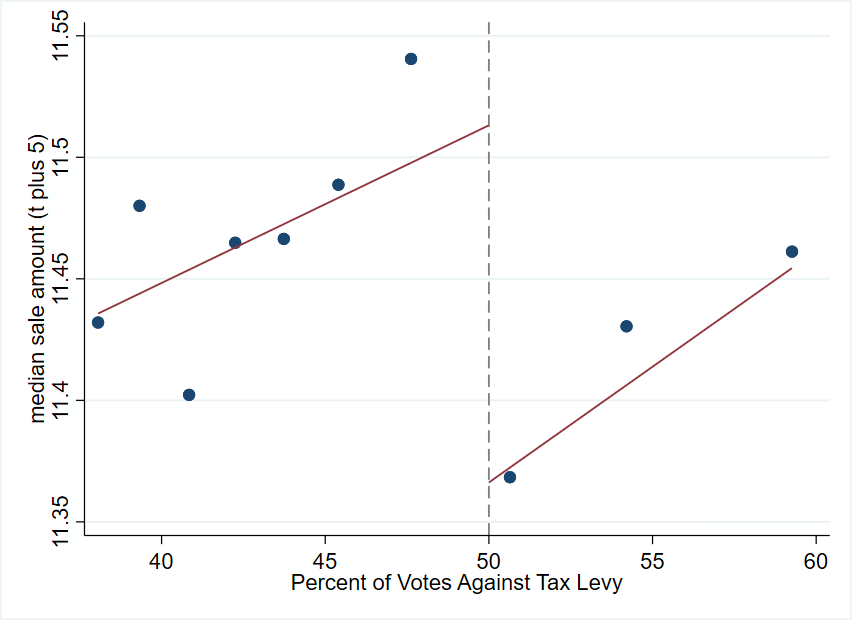
\includegraphics[width=\textwidth]{assets/imgs/rd_plot_median_sale_amount_t_plus_5_tri_mserd_1_2_within.png}
            \caption{Year 5 after vote}
        \end{minipage}
        \hfill
        \begin{minipage}[b]{0.35\textwidth}
            \centering
            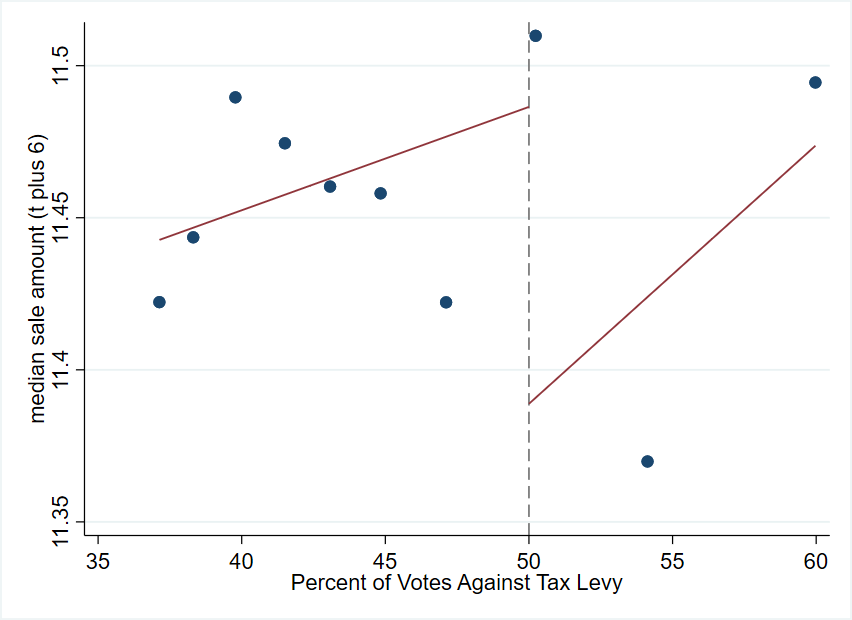
\includegraphics[width=\textwidth]{assets/imgs/rd_plot_median_sale_amount_t_plus_6_tri_mserd_1_2_within.png}
            \caption{Year 6 after vote}
        \end{minipage}
        \vspace{1em}
        \begin{minipage}[b]{0.35\textwidth}
            \centering
            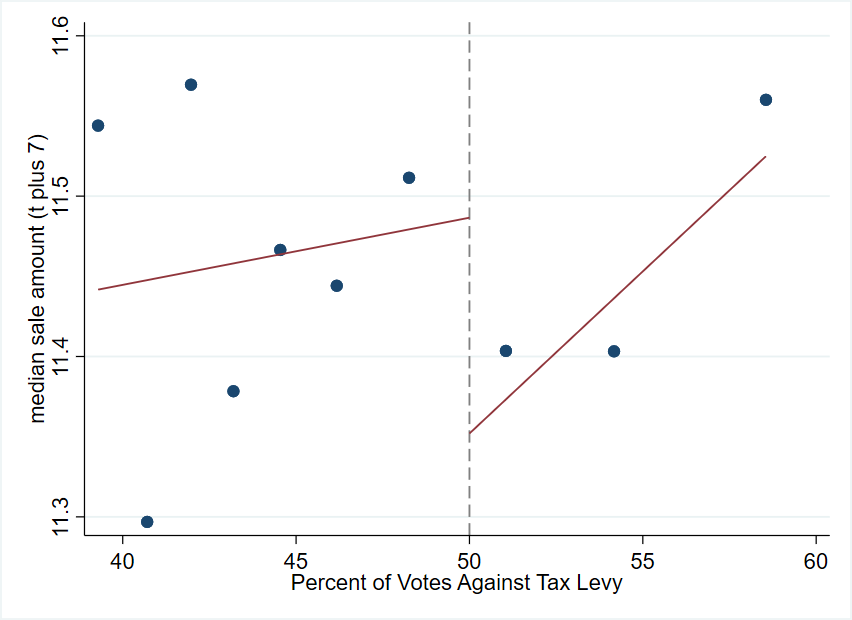
\includegraphics[width=\textwidth]{assets/imgs/rd_plot_median_sale_amount_t_plus_7_tri_mserd_1_2_within.png}
            \caption{Year 7 after vote}
        \end{minipage}
        \hfill
        \begin{minipage}[b]{0.35\textwidth}
            \centering
            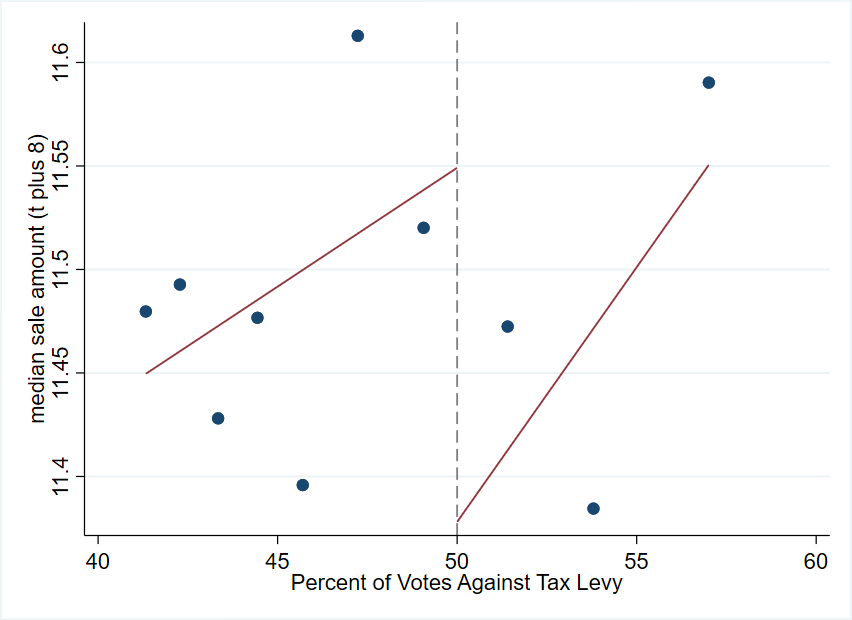
\includegraphics[width=\textwidth]{assets/imgs/rd_plot_median_sale_amount_t_plus_8_tri_mserd_1_2_within.png}
            \caption{Year 8 after vote}
        \end{minipage}
    \end{figure}
    
    \hyperlink{main_rd}{\beamerbutton{Housing Price: Main RD plot}}

\end{frame}

\begin{frame}[t]{Literature Review: People study roads}\vspace{10pt}
    \label{lit_background}    
    \begin{block}{Prior Econ Literature}
    JEL code {\bf R42}: Government and Private Investment Analysis • \textcolor{blue}{Road Maintenance} • Transportation Planning 
    \vspace{0.2cm}
    
    1. Asher and Novosad (2020) - 
    
    {\small
    {\bf Setting}: India 
    
    {\bf Policy}: Pradhan Mantri Gram Sadak Yojana (PMGSY) in 2000 
    
    {\bf Design}: Regression Discontinuity Design (RDD)
    
    {\bf Conclusion}: Limited causal effect on changes to employment in the village firms after 4 years, but large reallocation of labor out of agriculture.
    }
    
    \hyperlink{main_lit}{\beamerbutton{main literature}}
    
    \end{block}
    \end{frame}
    
    \begin{frame}[t]{Literature Review: People study roads}\vspace{1pt}
    \begin{block}{Prior Econ Literature}
    
    2. Yogita Shamdasani (2021) -
    
    {\small
    % {\bf Setting}: India 
    
    {\bf Policy}: Pradhan Mantri Gram Sadak Yojana (PMGSY) in 2000 
    
    {\bf Design}: Difference-in-Differences (DID)
    
    {\bf Conclusion}: New roads induce movement of workers out of agriculture for villages with access to non-agricultural sector. However, large gains in agricultural output for villages with little access to non-agricultural sector
    } 
    
    3. Ren Mu and Van De Walle (2010) -
    
    {\small
    
    {\bf Policy}: Rural Transport Project I (RTPI) in Vietnam
    
    {\bf Design}: Difference-in-Differences (DID)
    
    {\bf Conclusion}: It takes atleast 27 months to see any effect on economic development. Large increase in frequency of markets, primary school completion rates and households switch from agriculture to non-agriculture sector.
    }
    
\end{block}
\end{frame}
    

\begin{frame}{Tables}
\frametitle{}
\begin{table}[ht]
    \centering
    \caption{Effect on median house prices of failing to renew a road tax levy}
    \label{tab:median_sale_amount}
    \scriptsize % Make the text smaller
    \begin{tabular}{p{1.5cm}ccccccc}
        \hline
        \textbf{Year relative to vote} & \textbf{$t + 4$} & \textbf{$t + 5$} & \textbf{$t + 6$} & \textbf{$t + 7$} & \textbf{$t + 8$} & \textbf{$t + 9$} & \textbf{$t + 10$} \\
        \hline
        Treatment effect & -19,535 & -21,531 & -16,994 & -16,691 & -23,323 & -30,620 & -16,411 \\
        Standard error & (9,289) & (9,147) & (7,558) & (7,357) & (9,449) & (9,586) & (9,342) \\
        Effective bandwidth ($h$) & 8.9 & 12.1 & 14.1 & 14.0 & 8.2 & 8.2 & 8.3 \\
        Bias bandwidth ($b$) & 15.4 & 20.0 & 24.1 & 24.2 & 15.5 & 16.3 & 17.5 \\
        Effective Observations & 714 & 1,020 & 1,182 & 1,127 & 593 & 584 & 557 \\
        Total Observations & 2,618 & 2,535 & 2,442 & 2,328 & 2,204 & 2,119 & 2,022 \\
        \hline
    \end{tabular}
\end{table}
\end{frame}

\begin{frame}{}
\frametitle{}

\begin{table}[ht]
    \hspace{-1cm}
    % \centering
    \caption{Quantile-level Treatment Effects of Cutting Road Spending on Median House Prices}
    \label{tab:quantile_tes}
    \scriptsize % Make the text smaller
    \begin{tabular}{p{1cm}ccccccc}
        \hline
        Percentile & \textbf{$t + 4$} & \textbf{$t + 5$} & \textbf{$t + 6$} & \textbf{$t + 7$} & \textbf{$t + 8$} & \textbf{$t + 9$} & \textbf{$t + 10$} \\
        \hline
        10\% & -6,433 & -22,570 & -9,602 & -12,984 & -11,217 & -6,569 & -1,326 \\
        & (9,364) & (9,065) & (9,205) & (8,420) & (9,136) & (10,809) & (8,793) \\
        20\% & -5,400 & -15,070 & 4,014 & -14,682 & -15,040 & -3,228 & 624 \\
        & (9,983) & (9,886) & (7,443) & (8,502) & (8,160) & (10,435) & (8,509) \\
        70\% & -21,760 & -11,171 & -38,082 & -36,685 & -21,356 & -25,605 & -18,600 \\
        & (12,333) & (11,806) & (12,835) & (12,163) & (12,218) & (13,984) & (9,872) \\
        80\% & -28,478 & -16,379 & -38,460 & -37,470 & -28,950 & -27,800 & -18,658 \\
        & (13,343) & (11,404) & (18,623) & (12,169) & (12,507) & (12,421) & (11,808) \\
        90\% & -51,470 & -34,604 & -38,510 & -27,039 & -29,010 & -49,093 & -36,662 \\
        & (18,409) & (15,837) & (22,194) & (16,308) & (16,640) & (14,498) & (19,110) \\
        \hline
    \end{tabular}
\end{table}

\end{frame}


\end{document}

